\subsection{Durchführung des Versuchs}
In Abbildung~\ref{fig:stm1} sehen wir das RTM, welches in der
folgenden Versuchsdurchführung verwendet wurde. Es handelt sich
um das Modell \textit{easyScan 2 STM, Version 1.6} welches 
mittlerweile von 
der Firma \textit{Nanoscience Instruments, Ink.} vertrieben wird.
Laut der Beschreibung des Herstellers  
bilden hunderte \textit{easyScan 2 STMs} einen
\textit{unersetzlichen} Bestandteil in der Lehre von Physik,
Chemie und Materialwissenschaften, werden aber auch in der
Forschung und Entwicklung eingesetzt. Anwendung findet das RTM
in der Spektroskopie sowie in der Grundlagenforschung.
In unserem Versuch spielt das easyScan 2 STM insofern eine Rolle,
dass es ohne weitere Zwischeninstanzen direkt die gemessen
Abstände in ein Bild auf dem Computer sendet. Diese Bilder
enthalten schon alle für den Versuch notwendigen Informationen,
die Parameter können auch direkt von dem bereitgestellten Programm
konfiguriert werden. Der Wandel vom ersten RTM, in dem die Dämpfung
noch von Supraleitenden Magneten und einer Vakuumkammer hergestellt
werden musste, zum diesem Modell und diese Fortschritt kommt uns
in unserem FP zu Gute. Die Spezifikationen des Modells 
(Ausschnitt aus \cite{easyscan2_STM}):\\
\begin{table}[h]
\begin{tabular}{| l | p{7cm} |}
\hline
  Größe des Controllers, Gewicht: & 470x120x80 mm / 2.4 Kg\\ \hline
  Leistung & 90- 240 V~/ 30 W 50/60 Hz \\ \hline
  Rastergeschwindigkeit & Bis zu 60ms pro Linie mit 128 Datenpunkten  pro Linie \\ \hline
Rasterfläche & bis zu 2048x2048 Punkten \\ \hline 
Darstellungsmöglichkeiten: & Liniengraph, Farbplot und 3D Perspektive \\ \hline
Abbildungsmodi & Konstante Stromstärke (\textit{Constant Current}),
konstante Höhe (\textit{Constant Height}) \\ \hline
Maximale Auflösung in Z/ XY & 3pm/ 7.6pm \\ \hline
Maximaler Rasterumfang in Z/ XY & 200nm/ 500nm  \\ \hline
Maximale Probengröße & 10mm Durchmesser \\ \hline
Spitzenspannung & max. $\pm 10V$ in 5mV Schritten \\ \hline
\end{tabular}
\caption{Spezifikationen des Modells \textit{easyScan 2 STM} \cite{easyscan2_STM}}
\label{tab:STM}
\end{table}

\begin{figure}
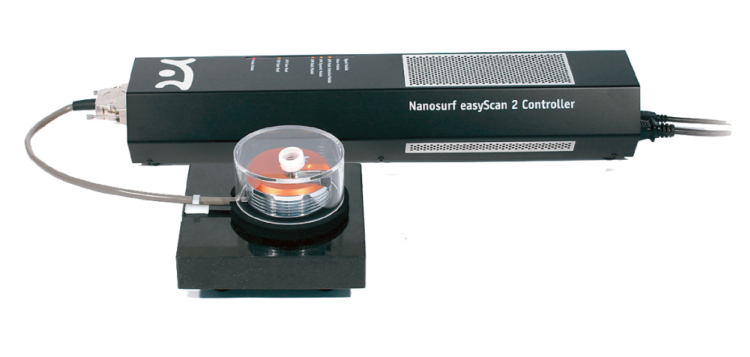
\includegraphics[width=14cm]{pics/stm1}
\caption{Photographie des verwendeten RTMs \textit{easyScan 2
STM} \cite{easyscan2_STM}} 
 \label{fig:stm1}
\end{figure}

Da die Messaparatur für unseren Versuch schon aufgebaut worden
war und nicht modifiziert werden sollte, werden wir hier nicht
auf die einzelnen Komponenten des \textit{easy Scan 2 STM} Systems
eingehen, sondern nur die für unseren Versuch relevanten 
Bauteile beschreiben.
\subsubsection{Versuchsaufbau}
In Abbildung~\ref{fig:Rasterkopf} ist der Rasterkopf ds RTMs zu
sehen. Über den Probenhalter mit dazugehörigem Fixierungsmagneten
wird die Probe selbst angebracht; an den Spitzenhalter mit
Klammer die Spitze aus Platin-Iridiumdraht, 
welche wir für die Messungen selbst herstellt haben (siehe
Abbildung~\ref{fig:prepare_tip} und Abbildung~\ref{SEM_tip_picture}).
Der Probehalter stellt einen Zylinder dar, an dessen Kopf mithilfe
eines Magneten die Probe, welche im Idealfall auf einer dafür
passenden, ebenfalls magnetischen Schablone angebracht ist, 
befestigt wird, nachdem die Spitze angebracht wurde. 
Das Anbringen der Spitze erfolgt mit dafür passenden Zangen,
indem die Klammer angehoben, die Spitze eingelegt und mit
der Klammer fixiert wird.

\begin{figure}
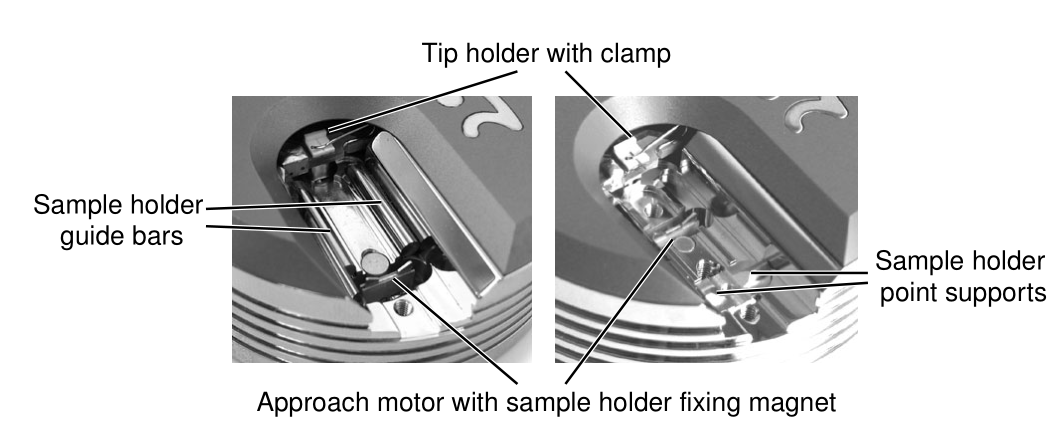
\includegraphics[width=14cm]{pics/rasterkopf}
\caption{Rasterkopf des RTMs \textit{easyScan 2
STM Version 1.6} \cite{easyscan2_STM}.
Zu Sehen ist der Probenhalter (\textit{Sample holder}) mit dazu
gehörendem Annäherungsmotor (\textit{Approach motor} sowie
dem Fixierungsmagneten ({Fixing Magnet}), sowie dem Spitzenhalter
mit Klammer (\textit{Tip holder with clamp}). Die Funktionsweise
wird im Text beschrieben.}
 \label{fig:Rasterkopf}
\end{figure}

\begin{figure}
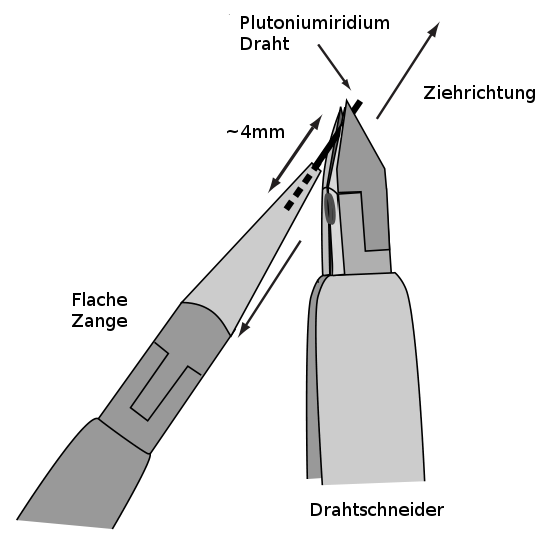
\includegraphics[width=10cm]{pics/prepare_tip2}
\caption{Vorbereitung des Drahtes. 1) Zunächst sollten die
zur Herstellung der Spitze notwendigen Werkzeuge mit Ethanol
gereinigt werden, von nun an sollte nur der Draht damit berührt 
werden. 2) Nun sollte der zu verknappende Draht mit den Zangen
gehalten werden, 3) dem Drahschneider umschlossen, aber nicht
abgezwickt, 4) in die angegebene Richtung \textbf{gezogen}, 5)
und endlich \textbf{abgerissen} werden, mit dem Ziel eine 
einatomige Spitze zu erzeugen (siehe Abbildung~\ref{fig:SEM_tip_picture})}
 \label{fig:prepare_tip}
\end{figure}

\begin{figure}
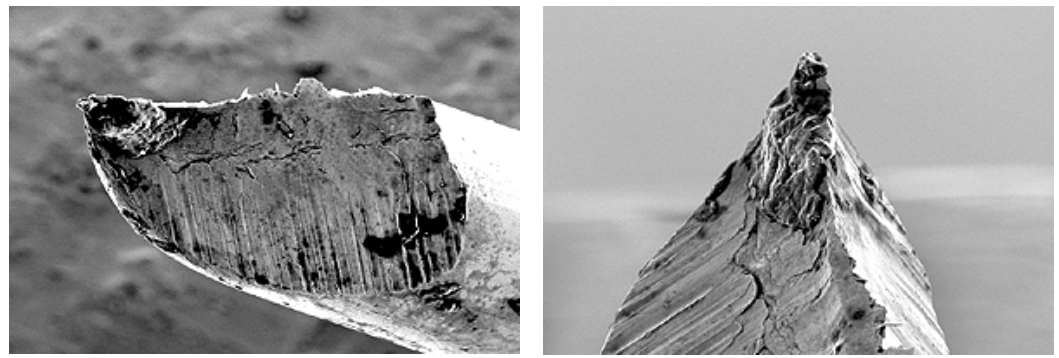
\includegraphics[width=10cm]{pics/SEM_tip_picture}
\caption{Das in Abbildung~\ref{fig:prepare_tip} beschriebene
Verfahren hat zum Ziel, eine möglichst präzise Spitze herzustellen.
Hier eine \textit{Scanning Electron Microskope} Abbildung
aus der Bedingungsanleitung des RTMs 
einer solchen hergestellen, idealen Spitze. Wie deutlich erkennbar
ist, verjüngt sich die Spitze nach oben und bietet so unter 
Umständen die Möglichkeit, eine einatomige Tunnelverbindung
mit der Probe einzugehen.}
 \label{fig:SEM_tip_picture}

\end{figure}
\subsubsection{Durchführung der Messungen}
Sobald die Spitze angebracht und die Probe eingeführt wurde, 
wird ein Plexiglasdeckel über die Apperatur aufgesetzt, welcher
über eine Luke mit einer Linse verfügt. Über jene Linse kann die
Distanz zwischen Probe und Spitze überprüft werden. Anschließend
kann der Annäherungsprozess der Spitze zu der Probe beginnen. 
Zunächst kann manuell mit einer groben Steuerung die Spitze
(visuell) so nah wie möglich an die Probe herangebracht werden.
Dabei ist es von Vorteil, wenn diese schon zu Beginn recht nahe
aneinander liegen. Danach startet man den automatischen
Annäherungsprozess,
der die Spitze solange mit einer jeweils eingestellten
Geschwindigkeit der Probe annähert, bis ein erster Tunnelstrom
(in der Regel 1 nA)
zwischen der Probe und der Spitze fließen kann.  
Dieser Annäherungsversuch verfügt über verschiedene Modi:
\begin{itemize}
    \item \textbf{\textcolor{orange}{orange}}:
            Der Annäherungsversuch ist noch
            nicht abgeschlossen
    \item \textbf{\textcolor{red}{rot}}: 
            Der Annäherungsversuch ist in dem Sinne
            gescheitert, dass die Spitze mit der Probe kollidiert
            ist und womöglich Schaden erlitten hat. 
    \item \textbf{\textcolor{green}{grün}}: 
            Der Annäherungsversuch
            wurde ohne Fehlermeldungen
            abgeschlossen und ist vermutlich geglückt;
            der Tunnelstrom fließt wie vorgegeben.
\end{itemize}
Der erste Annäherung genügt in der Regel nicht, die Probe
mit der gewünschten Auflösung betrachten zu können. Deswegen muss
sukzessiv die Distanz 
durch weitere Annäherungen verkleinert werden,
unter jeweils niedrigerer
Tunnelspannung und veringerter Annäherungsgeschwindigkeit, 
ohne dass dabei die Spitze mit der Probe kollidiert.
Wenn nun die Annäherung erfolgt ist, kann die Abrasterung
der Probe beginnen. Die Qualität des Kontakts zwischen Probe
und Spitze kann nun anhand verschiedener Kriterien beurteilt werden,
darunter die der Spitze umgebende Höhenlinie (siehe
Abbildung~\ref{fig:topography}).
\begin{figure}
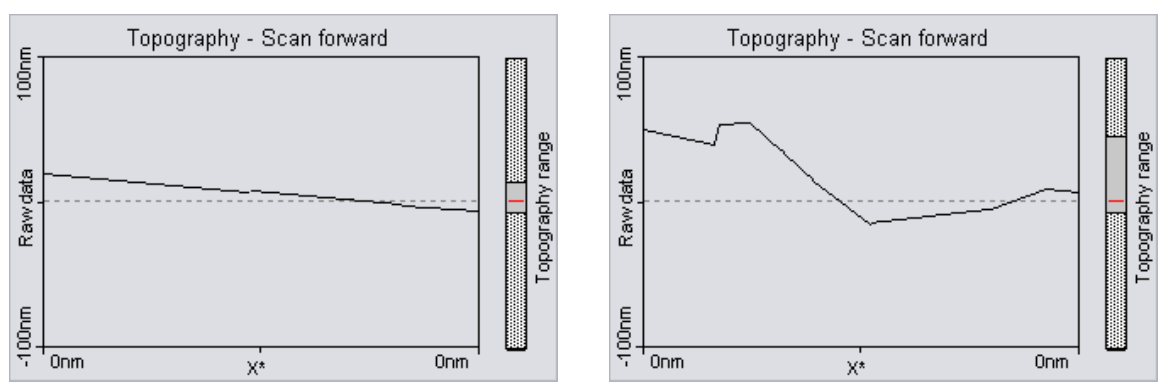
\includegraphics[width=14cm]{pics/Topography}
\caption{Screenshot aus dem Programm \cite{easyscan2_STM}. 
Links zeigt eine 
Topographische Linie für einen guten Kontakt, während die
rechte ``nervöse'' Linie aufgrund ihrer Nichtlinearität
einen schlechten Tunneling Kontakt
andeutet, was auf eine zu stumpfe oder instabile Spitze
zurückgeführt werden kann.}
 \label{fig:topography}
\end{figure}
Wenn nun eine erfolgreiche Abrasterung mit zufriedenstellender
Auflösung vorliegt, kann ein Ausschnitt der Abrasterung
vergrößert werden (siehe Abbildung~\ref{fig:zoom});
dieser Auschnitt wird dann erneut abgerastert
(sofern die technisch mögliche Auflösung nicht überschritten wird,
siehe Tabelle~\ref{tab:STM} auf Seite~\pageref{tab:STM}).
Wie gut die Auflösung effektiv ist, hängt von der Qualität der 
Spitze, den Parametern (Messzeit pro Linie, Regeparameter des
PID-Controllers, Spannung am Tunnelstrom) und dem Einfluss durch
äußere Gegebenheiten (Rauschen durch Geräusche, usw.) ab. 
Durch Überprüfung, ob vorwärz- und rückwärts-Rasterung,
Änderung der Messzeit pro Linie, Veränderung des Tunnelstroms,
oder Abrasterung derselben Stelle mehrere Male  
dasselbe Ergebnis liefern, oder ob Rotation der Rasterichtung
um $90^{\circ}$ korrekt abgebildet wird, kann überprüft werden,
ob die Auflösung gut ist \cite{versuchsanleitung}.
Bei periodischen Strukturen kann überprüft werden, ob eine
Veränderung der Messzeit pro Linie die Periodizität beeinflusst
\cite{versuchsanleitung}. Wenn abschließend die gewünschten
Messungen vorgenommen wurden, kann mit der Auswertung 
durch Bildanalyseverfahren begonnen werden. 
\begin{figure}
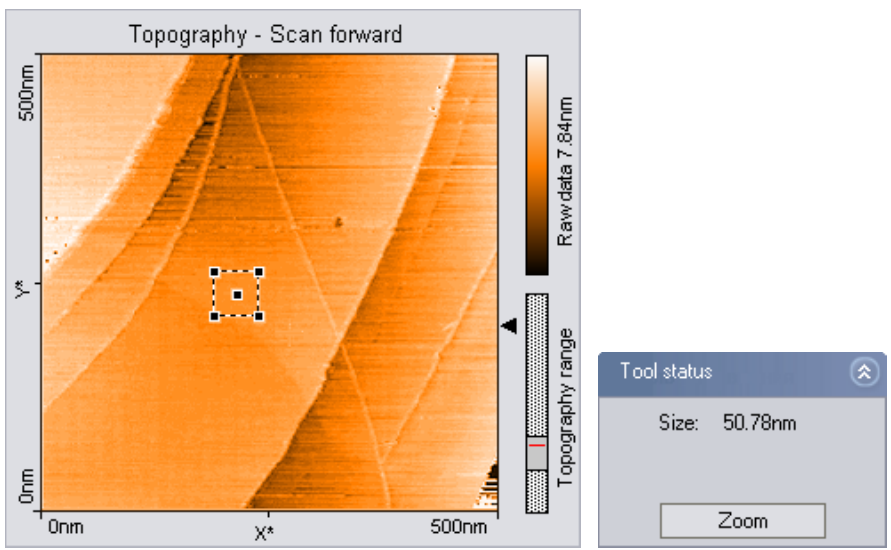
\includegraphics[width=14cm]{pics/zoom}
\caption{Screenshot aus dem Programm \cite{easyscan2_STM}.
Hier wurde eine rechteckige Auswahl von 50.78nm Seitenlänge
getroffen, diese wird nun unter weiterer Rasterung vergrößert.}
 \label{fig:zoom}
\end{figure}


\subsubsection{Analysesoftware Gwyddion}
Bei der Analysesoftware Gwyddion handelt es sich um ein modulares
Programm für Rastersondenmikroskopie (\textit{scanning probe
microskopy}, \textbf{STM}) 
im Allgemeinen \cite{gwyddion}, unter anderem auch für RTMs.
Es unterstützt viele verschiedene STM-Formate (50 verschiedene)
und verfügt über zahlreiche Analysemethoden, 
um Höhenfelder, wie sie das RTM erzeugt,
auszuwerten. Gwyddion ist kostenlos und Open Source software,
programmiert unter der \textit{GNU General Public License (GPL)}.
Es ist verfügbar für GNU/Linux, Microsoft Windows, Mac OS X und
FreeBSD Betriebssysteme\cite{gwyddion}.
Die Funktionalität erstreckt sich unter anderem über:
\begin{itemize}
    \item OpenGl 3D Ansicht in Falschfarben
    \item Kanten- und Gradientenerkennung (u.a. Laplacefilter und andere diskrete Faltungen)
    \item Integraltransformationen (2D FFT, Wavelet transform, usw.)
    \item Datenanalyse unter der Benutzung von neuronalen Netzen
\end{itemize}
Die genaue Funktionsweise soll hier nicht beschrieben werden
und kann der Webseite\cite{gwyddion} entnommen werden.


\begin{figure}
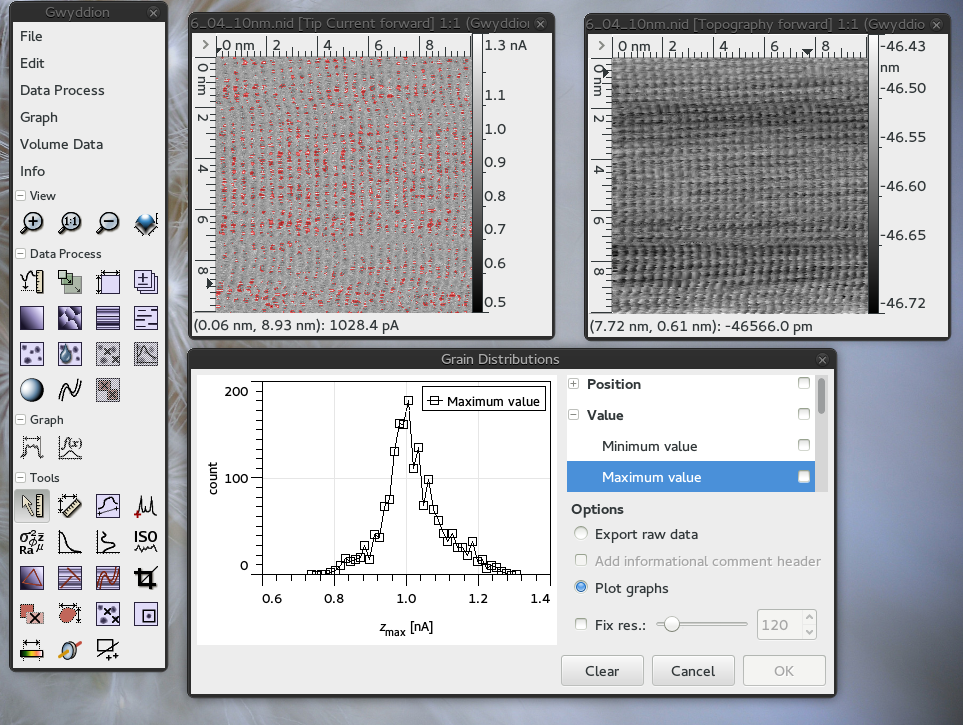
\includegraphics[width=18cm]{pics/gwyddion_screenshot}
\caption{Screenshot des Analyseprogramms Gwyddion, welches
auf der Webseite frei verfügbar ist\cite{gwyddion}.}
 \label{fig:gwyddion_screenshot}

\end{figure}
